\section{Existence and Uniqueness Results for Ordinary Fractional Differential Equations}
In this section we establish some analytical results for ordinary fractional differential equations. These results allow us to solve some simple initial value problems and establish a theoretical framework from which results in other sections can draw.

We will first outline a set of ideas which can guarantee the existence of a solution to an initial value problem involving fractional derivatives. These ideas are outlined in \cite{Tisdell2012} but we present these ideas here because they form the basis for a generalisation we would like to present in theorem \ref{thm-existence-uniq}.

\begin{mdframed}[innertopmargin=10pt]
\begin{propdef}
    Let $ \beta > 0, \alpha > 0 $ and $ a > 0 $. For $ x,y \in C([0,a]) $ the function
    \begin{align*}
        d_{\beta}(x,y) := \max_{t \in [0,a]} \frac{|x(t) - y(t)|}{E_{\alpha,1}(\beta t^\alpha)}
    \end{align*}
    defines a metric on the space of functions $ C([0,a]) $. 
\end{propdef}
\end{mdframed}

This metric, as presented by Tisdell, \cite{Tisdell2012}, is a generalisation of the Bielecki metric \cite{Tisdell2012, Bielecki1956}. 

\begin{proof}
    It is well known that $ d(x,y) = \max_{t \in [0,a]}|x(t) - y(t)| $ defines a metric on $C([0,a]) $. Now it is easy to see that for $ t > 0 $, $ E_{\alpha,1}(\beta t^\alpha) >0 $. It is also well known that $ E_{\alpha,1}(t) $ is continuous on $ [0, a] $ so it follows that $ d_{\beta}(x,y) $ is a metric.
\end{proof}

\begin{mdframed}[innertopmargin=10pt]
\begin{lemma}
    The metric space $ (C([0,a]), d_\beta) $ is complete.
\end{lemma}
\end{mdframed}
\begin{proof}
    We only have to show that $ d_\beta $ is equivalent to the max metric ($ d(x,y) = \max_{t \in [0,a]}|x(t) - y(t)| $) to get this result because it is well known that $ (C([0,a]), d) $ is a complete metric space.
    It is easy to see that $ E_{\alpha, 1}(\beta t^\alpha) $ is strictly increasing on $ [0, a] $ and so 
    \begin{align}
        \frac{1}{E_{\alpha, 1}(\beta t^\alpha)} d(x,y) \leq d_\beta(x,y) \leq d(x,y).
    \end{align}
    This shows that the metrics are equivalent and hence $ (C([0,a]), d_\beta) $ is complete.
\end{proof}

Using these definitions and results we can now say something about the existence and uniqueness of solutions to an initial value problem. The following lemma is from Tisdell \cite{Tisdell2012}. Our proof is also the same, but with more justifications for each step. These justifications are important as they will be required somewhat more in the proof of theorem \ref{thm-existence-uniq}.

\begin{mdframed}[innertopmargin=10pt]
\begin{theorem}[Uniqueness]
    \label{thm:unique-tisdell}
    Consider the initial value problem 
    \begin{align}
        \label{eq:ivp_uniq_1}    
        \prescript{C}{0}{\mathcal{D}}x(t) = f(t,x(t))
    \end{align}
    \begin{align}
        \label{eq:ivp_uniq_ic_1}
        x(0) = a_0, x'(0) = a_1, \ldots, x^{(n-1)}(0) = a_{n-1}.
    \end{align}
    Let 
	\begin{align*}
	    S:= \{ (t,p) \in \Rl^2 : t \in [0, a], p \in \Rl \} 
	\end{align*}
	and let $ f : S \lra \mathcal{R} $ be continuous. If there is a positive constant $ L $ such that 
	\begin{align}
		\label{eq:ivp_uniq_1_lipshitz}
	    |f(t,u) - f(t,v)| \leq L|u-v| 
	\end{align}   
	for all $ (t,u), (t,v) \in S $
	then \eqref{eq:ivp_uniq_1} and \eqref{eq:ivp_uniq_ic_1} has a unique solution on $ [0, a] $.
\end{theorem}
\end{mdframed}
\begin{proof}
	Choose $ \beta $ so that $ \frac{L}{\beta} < 1 $.
	\begin{align*}
		d_\beta(x,y) = \max_{t \in [0,a]} \frac{|x(t) - y(t)|}{E_{\alpha,1}(\beta t^\alpha)}
	\end{align*}
	combined with the space $ C([0,a]) $ forms a complete metric space. By applying $ I_0^\alpha $ to both sides of \eqref{eq:ivp_uniq_1} and applying lemma \ref{lem:rli-cap} we get that \eqref{eq:ivp_uniq_1} and \eqref{eq:ivp_uniq_ic_1} are equivalent to the integral equation
	\begin{align}
		\label{eq:ivp_1_int}
		x(t) = \sum_{k=0}^{n-1} \frac{a_k t^k}{k!} + \frac{1}{\Gamma(\alpha)} \int_0^t (t-s)^{\alpha-1}f(s,x(s))ds
	\end{align}
	for $ t \in [0,a] $.
	The idea is to prove that the right hand side of \eqref{eq:ivp_1_int} is a contraction in the space $ (C([0,a]),d_\beta) $. By (an immediate corollary to) Banach's fixed point theorem this shows the existence of a unique solution to the integral equation, and hence the IVP defined in \eqref{eq:ivp_uniq_1} and \eqref{eq:ivp_uniq_ic_1}.
	Define $ F : C([0,a]) \lra C([0,a]) $
	as
	\begin{align*}
		[Fx](t) = \sum_{k=0}^{n-1} \frac{a_k t^k}{k!}  + \frac{1}{\Gamma(\alpha)} \int_0^t (t-s)^{\alpha-1}f(s,x(s))ds.
	\end{align*}
	For any $ x, y \in C([0,a]) $ and consider
	\begin{align*}
		d_\beta(Fx,Fy) &= \max_{t\in[0,a]} \frac{|[Fx](t) - [Fy](t)|}{E_{\alpha,1}(\beta t^\alpha)} \\
			&\leq \max_{t\in[0,a]} \left[ \frac{1}{E_{\alpha,1}(\beta t^\alpha)} \frac{1}{\gamma(\alpha)} \int_0^t (t-s)^{\alpha-1}| f(s,x(s)) - f(s,y(x))|ds  \right]
	\end{align*}
	and by using the Lipschitz condition in \eqref{eq:ivp_uniq_1_lipshitz} we get that
	\begin{align*}
		d_\beta(Fx,Fy) &\leq \max_{t\in[0,a]} \left[ \frac{1}{E_{\alpha,1}(\beta t^\alpha)} \frac{1}{\Gamma(\alpha)} \int_0^t (t-s)^{\alpha-1}L| x(s) - y(x)|ds  \right] \\
		&= L  \max_{t\in[0,a]} \left[ \frac{1}{E_{\alpha,1}(\beta t^\alpha)} \frac{1}{\Gamma(\alpha)} \int_0^t (t-s)^{\alpha - 1} E_{\alpha,1}(\beta s^\alpha) \frac{|x(s) - y(s)|}{E_{\alpha,1}(\beta s^\alpha)} ds \right] \\
		&\leq \underbrace{L d_\beta(x,y) \max_{t\in [0,a]} \left[ \frac{1}{E_{\alpha,1}(\beta t^\alpha)}\frac{1}{\Gamma(\alpha)} \int_0^t (t-s)^{\alpha-1} E_{\alpha,1}(\beta s^\alpha) ds\right]}_{\circledast}
	\end{align*}
	Now noticing the fractional integral we have that
	\begin{align*}
		\circledast &= L d_\beta(x,y) \max_{t\in [0,a]} \left[ \frac{1}{E_{\alpha,1}(\beta t^\alpha)} I^\alpha_0 E_{\alpha,1}(\beta s^\alpha) \right]
	\end{align*}
	by using the result of lemma \ref{lem-rli-mit-lef-2} we have that
	\begin{align*}
		\circledast &= L d_\beta(x,y) \max_{t\in [0,a]} \left[ \frac{1}{E_{\alpha,1}(\beta t^\alpha)} \left( \frac{E_{\alpha,1}(\beta z^\alpha) - 1}{\beta} \right) \right] \\
			&= L d_\beta(x,y) \max_{t\in [0,a]} \frac{1}{\beta}\left[ 1 - \frac{1}{E_{\alpha, 1}(\beta t^\alpha)} \right].
	\end{align*}
	From the definition of $ E_{\alpha,1} $ it should be clear to see that $ E_{\alpha, 1}(\beta t^\alpha) $ is monotonically increasing for $ t \geq 0 $ and so
	\begin{align*}
		\circledast &= \frac{L}{\beta} d_\beta (x,y)\left[ 1- \frac{1}{\beta a^\alpha} \right]
	\end{align*}
	and hence by the assumption that $ \frac{L}{\beta} < 1 $ we have that $ \circledast < 1 $ and hence $ d_\beta(Fx, Fy) < d_\beta(x,y) $ and so the right hand side of \eqref{eq:ivp_1_int} is a contraction and thus by (an immediate corollary to) Banach's fixed point theorem \eqref{eq:ivp_1_int} has a unique solution on $ [0,a] $.
\end{proof}



The following theorem generalizes the result above by Tisdell \cite{Tisdell2012} but a similar result for Miller-Ross sequential
fractional differential equations can be found in \cite{Podlubny1999}.

\begin{mdframed}[innertopmargin=10pt]
\begin{theorem}[Uniqueness]
\label{thm-existence-uniq}
Consider the following intial value problem,

	\begin{align}
		\label{eq-fde-ivp-1}
		\sum_{j=1}^{N} \beta_j\capder{0}{t}{\alpha_j}{x}(t) = f(t,x(t)) \\
		\label{eq-fde-ivp-ic-1}
		x(0) = A_0, x_1(0) = A_1, \ldots, x^{n_N}(0) = A_{n_N}
	\end{align}
	where $ \alpha_1 > \alpha_2 > \ldots > \alpha_N $.
	
	Define
		\begin{align*}
		 S:= \{ (t,p) \in \Rl^2 : t \in [0, a], p \in \Rl \} 
		\end{align*}
	Let $ f : S \lra \Rl $ be continuous. If there is a positive constant L such that 
		\begin{align}
		\label{eq:uniq-lipshitz}
		|f(t,u) - f(t,v)| \leq L|u-v|, \text{ for all } (t,u), (t,v) \in S
		\end{align}
and the set of constants $ \{ \alpha_j \}_{j = 1}^{N} $, $ \{ \beta_j \}_{j=1}^N $
such that we can choose $ \gamma $ sufficiently large such that the following holds on $ [0, a] $
	\begin{align}
	    \label{eq:fde-uniq-cond}
\sum_{j=2}^N |\beta_j| a^{\alpha_1 - \alpha_j} \frac{E_{\alpha_1,1+\alpha_1-\alpha_j}(\gamma t^{\alpha_1})}{E_{\alpha_1,1}(\gamma t^{\alpha_1})} < 1
	\end{align}
	then the intial value problem defined in \ref{eq-fde-ivp-1} and \ref{eq-fde-ivp-ic-1} has a unique solution on $ [0, a] $.
\end{theorem}
\end{mdframed}
To prove this we will need two lemmas. 
\begin{mdframed}[innertopmargin=10pt]
\begin{lemma}
	The IVP defined in \eqref{eq-fde-ivp-1}, \eqref{eq-fde-ivp-ic-1} is equivalent to the integral equation
	\begin{align}
		\label{eq:equiv_int_2}
		x(t) &= \sum_{k=1}^{n_1}\frac{A_kt^k}{k!} + \frac{1}{\beta_1} \Bigl( \frac{1}{\Gamma(\alpha_1)}\int_{0}^{t} (t-s)^{\alpha_1 - 1}f(s,x(s))ds \\
			& \ \ \ - \sum_{j=2}^{N}\beta_j \frac{1}{\Gamma(\alpha_1 - \alpha_j)}
			\int_{0}^{t}(t-s)^{\alpha_1 - \alpha_j - 1}\left(x(s) - \sum_{k=1}^{n_j}\frac{A_ks^k}{k!} \right) ds \Bigr)
	\end{align}
\end{lemma}
\end{mdframed}
\begin{proof}
	Apply $ I_0^{\alpha_1} $ to both sides of \eqref{eq-fde-ivp-1} and then apply lemma \ref{lem:rli-cap}. Alternatively apply lemma \ref{lem:cap_rli} to either side of \eqref{eq:equiv_int_2}. 
\end{proof}

\begin{mdframed}[innertopmargin=10pt]
\begin{lemma}
\label{lem-rli-mit-lef-1}
For $ \xi > 0 $, $ \gamma > 0 $ and $ \alpha > 0 $ we have that
	\begin{align*}
		{I}^\xi_0 E_{\alpha,1}(\gamma t^\alpha) = t^\xi E_{\alpha,1+\xi}(\gamma t^\alpha).
	\end{align*}
\end{lemma}
\end{mdframed}
\begin{proof}
	This can be proved rather easily with Laplace transform methods.
	By using the results of lemmas \ref{lem:rli_laplace} and \ref{lem:lap_mit} we have that
	\begin{align}
	    \mathcal{L}\{ I_0^\xi E_{\alpha, 1}(\gamma t^\alpha) \} = \frac{s^{\alpha-\xi-1}}{s^\alpha - \gamma}
	\end{align}
	then by inverting the with the help of lemma \ref{lem:lap_mit_2} we have the result.
\end{proof}

\begin{proof}[Proof of theorem \ref{thm-existence-uniq}]

	To arrive at this we only have to prove that the map
	\begin{align*}
		[Fx](t) &:= \sum_{k=1}^{n_1}\frac{A_kt^k}{k!} + \frac{1}{\beta_1} \Bigl( \frac{1}{\Gamma(\alpha_1)}\int_{0}^{t} (t-s)^{\alpha_1 - 1}f(s,x(s))ds \\
			& \ \ \ - \sum_{j=2}^{N} \frac{\beta_j}{\Gamma(\alpha_1 - \alpha_j)}\int_{0}^{t}(t-s)^{\alpha_1 - \alpha_j - 1}\left(x(s) - \sum_{k=1}^{n_j}\frac{A_ks^k}{k!} \right) ds \Bigr)
	\end{align*}
	is contractive in the metric space $ \left( C[0,a], d^{\alpha_1}_\gamma \right) $  where 
	$$ d_\gamma^{\alpha_1}(x,y) = \max_{t \in [0, a]} \frac{|x(t) - y(t)|}{E_{\alpha_1,1}(\gamma t^{\alpha_1})}. $$
	To see this note that
	\begin{align*}
		d_\gamma^{\alpha_1}(Fx,Fy) &= \max_{t \in [0, a]}  \frac{1}{E_{\alpha_1}(\gamma t^{\alpha_1})} 
			\left| \frac{1}{\beta_1} \right| \Bigl| \frac{1}{\Gamma(\alpha_1)}\int_0^t (t-s)^{\alpha_1 - 1} (f(s,x(s)) - f(s,y(s))ds \\ 
			& \ \ \ - \sum_{j=2}^N \frac{\beta_j}{\Gamma(\alpha_1 - \alpha_j)} \int_0^t (t-s)^{\alpha_1 - \alpha_j - 1}(x(s) - y(s)) ds \Bigr| \\
			&\leq \max_{t \in [0, a]} \frac{1}{E_{\alpha_1}(\gamma t^{\alpha_1}) | \beta_1 |} \Big(
			 \frac{1}{\Gamma(\alpha_1)}\int_0^t (t-s)^{\alpha_1 - 1} |f(s,x(s)) - f(s,y(s))|ds \\ 
			& \ \ \ + \sum_{j=2}^N \frac{|\beta_j|}{\Gamma(\alpha_1 - \alpha_j)} \int_0^t (t-s)^{\alpha_1 - \alpha_j - 1}|x(s) - y(s))| ds \Bigr).
	\end{align*}
	By exploiting the Lipshitz condition \eqref{eq:uniq-lipshitz} we can further write that 
	\begin{align*}
		d_\gamma^{\alpha_1}(Fx,Fy) &\leq \max_{t \in [0, a]} \frac{1}{E_{\alpha_1}(\gamma t^{\alpha_1})|\beta_1|} \Bigl(
			\frac{L}{\Gamma(\alpha_1)}\int_0^t (t-s)^{\alpha_1 - 1} |x(s) - y(s)|ds \\ 
			& \ \ \ + \sum_{j=2}^N \frac{|\beta_j|}{\Gamma(\alpha_1 - \alpha_j)} \int_0^t (t-s)^{\alpha_1 - \alpha_j - 1}|x(s) - y(s))| ds \Bigr) \\
			&= \max_{t \in [0, a]} \frac{1}{E_{\alpha_1}(\gamma t^{\alpha_1})|\beta_1|} \Bigl(
			\frac{L}{\Gamma(\alpha_1)}\int_0^t (t-s)^{\alpha_1 - 1} \frac{|x(s) - y(s)|}{E_{\alpha_1}(\gamma s^{\alpha_1})}E_{\alpha_1}(\gamma s^{\alpha_1})ds \\ 
			& \ \ \ + \sum_{j=2}^N \frac{|\beta_j|}{\Gamma(\alpha_1 - \alpha_j)} \int_0^t (t-s)^{\alpha_1 - \alpha_j - 1}\frac{|x(s) - y(s))|}{E_{\alpha_1}(\gamma s^{\alpha_1})}E_{\alpha_1}(\gamma s^{\alpha_1}) ds \Bigr) \\
			&\leq d_\gamma^{\alpha_1}(x,y) \max_{t \in [0, a]} \frac{1}{E_{\alpha_1}(\gamma t^{\alpha_1})|\beta_1|} \Bigl(
			\frac{L}{\Gamma(\alpha_1)}\int_0^t (t-s)^{\alpha_1 - 1} E_{\alpha_1}(\gamma s^{\alpha_1}) ds \\
			& \ \ \ + \sum_{j=2}^N \frac{|\beta_j|}{\Gamma(\alpha_1 - \alpha_j)} \int_0^t (t-s)^{\alpha_1 - \alpha_j - 1}E_{\alpha_1}(\gamma s^{\alpha_1}) ds \Bigr) \\
			&= d_\gamma^{\alpha_1}(x,y) \max_{t \in [0, a]} \frac{1}{E_{\alpha_1}(\gamma t^{\alpha_1})|\beta_1|} \Bigl(
			L \rli{0}{\alpha_1}{E_{\alpha_1}(\gamma t^{\alpha_1}} \\
			& \ \ \ + \sum_{j=2}^N |\beta_j| \rli{0}{\alpha_1 - \alpha_j}{E_{\alpha_1}(\gamma t^{\alpha_1})} \Bigr). \\
	\end{align*}
	We can now use the results of lemmas \ref{lem-rli-mit-lef-1} and \ref{lem-rli-mit-lef-2} to write
	\begin{align*}
		d_\gamma^{\alpha_1}(Fx,Fy) &\leq d_\gamma^{\alpha_1}(x,y) \max_{t \in [0, a]} \frac{1}{E_{\alpha_1, 1}(\gamma t^{\alpha_1})|\beta_1|} \Bigl(
			\frac{L}{\gamma}\left( E_{\alpha_1,1}(\gamma t^{\alpha_1}) - 1 \right) \\
			& \ \ \ + \sum_{j=2}^N |\beta_j| t^{\alpha_1 - \alpha_j} E_{\alpha_1, 1 + \alpha_1 - \alpha_j}(\gamma t^{\alpha_1}) \Bigr) \\
			&= d_\gamma^{\alpha_1}(x,y) \max_{t \in [0, a]} \frac{1}{|\beta_1|} \Bigl(
			\frac{L}{\gamma}\left( 1- \frac{1}{E_{\alpha_1}(\gamma t^{\alpha_1})} \right) + \sum_{j=2}^N |\beta_j| t^{\alpha_1 - \alpha_j}\frac{E_{\alpha_1,1+\alpha_1-\alpha_j}(\gamma t^{\alpha_1})}{E_{\alpha_1,1}(\gamma t^{\alpha_1})}\Bigr) \\
	\end{align*}
	and finally we get that 
	\begin{align*}
		d_\gamma^{\alpha_1}(Fx,Fy) &\leq d_\gamma^{\alpha_1}(x,y) \frac{1}{|\beta_1|}\left( \frac{L}{\gamma} + \sum_{j=2}^N |\beta_j| a^{\alpha_1 - \alpha_j} \frac{E_{\alpha_1,1+\alpha_1-\alpha_j}(\gamma t^{\alpha_1})}{E_{\alpha_1,1}(\gamma t^{\alpha_1})} \right).
	\end{align*}
	By choosing $ \gamma $ sufficiently large we get that 
	$$
		\frac{1}{|\beta_1|}\left( \frac{L}{\gamma} + \sum_{j=2}^N |\beta_j| a^{\alpha_1 - \alpha_j} \frac{E_{\alpha_1,1+\alpha_1-\alpha_j}(\gamma t^{\alpha_1})}{E_{\alpha_1,1}(\gamma t^{\alpha_1})} \right) < 1
	$$
	and so $ F $ is a contractive mapping and thus the IVP defined in \eqref{eq-fde-ivp-1}, \eqref{eq-fde-ivp-ic-1} has a unique solution on $ [0, a] $.
\end{proof}

This result could be improved by removing the condition  in \eqref{eq:fde-uniq-cond}. This can be done in the case of $ 0 < \alpha < 2 $ because we can use lemma \ref{lem:mit_lef_asym_exp_1}. For this let us state and prove the following lemma.

\begin{mdframed}[innertopmargin=10pt]
\begin{lemma}
	\label{lem:mit_lef_quotient}
	For $ 0 < \alpha < 2 $, $ \beta > 0 $ and $ \varepsilon > 0 $ we have
	\begin{align}
		\lim_{z \lra \infty} \frac{E_{\alpha, \beta + \varepsilon}(z)}{E_{\alpha, \beta}(z)} = 0.
	\end{align}
\end{lemma}
\end{mdframed}

\begin{proof}
	Using lemma \ref{lem:mit_lef_asym_exp_1} we have that since $ z \in G^+ $,
	\begin{align*}
		\lim_{z \lra \infty} \frac{E_{\alpha, \beta + \varepsilon}(z)}{E_{\alpha, \beta}(z)} &= \lim_{z \lra \infty}\frac{\frac{1}{\alpha} z^{(1 - \beta - \varepsilon) / \alpha} e^{z^{1/\alpha}} - \sum_{k=1}^p \frac{z^{-k}}{\Gamma(\beta + \varepsilon - \alpha k)} + O(|z|^{-1-p})}{\frac{1}{\alpha} z^{(1 - \beta) / \alpha} e^{z^{1/\alpha}} - \sum_{k=1}^p \frac{z^{-k}}{\Gamma(\beta - \alpha k)} + O(|z|^{-1-p})}
	\end{align*}
	for some arbitrary integer $ p > 0 $.
	With sufficiently many applications of L'Hopital's rule we are left with
	\begin{align*}
		\lim_{z\lra\infty} z^{\frac{-\varepsilon}{\alpha}}		
	\end{align*}
	which is clearly equal to zero.
	Some care must be taken if we choose $ \beta $, $ \alpha $, and $ \varepsilon $ such that $ \beta - \alpha k $ or $ \beta + \varepsilon - \alpha k $ are ever integers due to singularities in the Gamma function, but it should be clear that these issues do not \emph{break} the argument as we could just regard those terms in the sums for which this does occur as $ 0 $.
\end{proof}

Interestingly this limit converges \emph{very} slowly for some choices of $ \alpha, \beta, \varepsilon $. Figure \ref{fig:mittag-quotient} gives an good illustration of this slow convergence.

\begin{figure}[H]
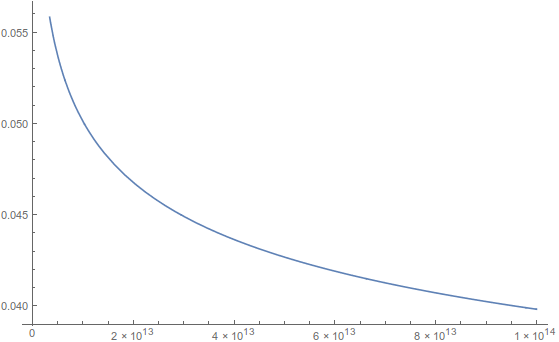
\includegraphics[scale=0.6]{images/Mittag-Leffler-Quotient}
\caption{$ E_{\alpha, \beta + \varepsilon}(z) / E_{\alpha, \beta}(z) $ for $ \alpha = 1, \beta = 1 $ and $ \varepsilon = 0.1 $.}
\label{fig:mittag-quotient}
\end{figure}

It should be clear that if $ \alpha_1 < 2 $ then the conditions in \ref{eq:fde-uniq-cond} is fulfilled and so we can \emph{always} choose a $ \gamma $ large enough that \eqref{eq:fde-uniq-cond} holds.


Both theorems \ref{thm:unique-tisdell} and \ref{thm-existence-uniq} are important as they give us some guarentees about the existance and uniqueness of solutions the initial value problems involving fractional derivatives. The generalisation in \ref{thm-existence-uniq} is important as it could be applied to showing the existance of solutions equations like the Bagley-Torvick equation which is a multi-order fractional differential equation that models the motion of a plate in a viscus fluid \cite{Diethelm2002-3, Podlubny1999, Torvik1984}.

In fact these results can be taken quite a bit further. The proof techniques used in theorems \ref{thm:unique-tisdell} and \ref{thm-existence-uniq} suggest a constructive method for arriving at a solution to fractional differential equations. This is formalised by Tisdell \cite{Tisdell2012} through the method of successive approximations. A similar idea is also outlined in \cite{Podlubny1999}.

\subsection{A generalised Gronwall's Inequality}

There are obviously other techniques for guaranteeing uniqueness, or non-multiplicity, to solutions, many of these are outlined in \cite{Tisdell2012} and \cite{Podlubny1999}. We would like to present here a result that hinges off a \emph{generalised Gronwall's inequality}. The \emph{generalised Gronwall's inequality}  was shown by Diethlem \cite{Diethelm2004_2}.

\begin{mdframed}[innertopmargin=10pt]
\begin{lemma}[Generalised Gronwall's Inequality]
	\label{lem:gronwall}
	Let $ a, A, B $ and $ C $ all be non-negative real constants and let $ \rho:[0,a] \lra [0, \infty) $ be continuous. If
	\begin{align*}	
		\rho(t) \leq A + \frac{1}{\Gamma(\alpha)} \int_0^t (t-s)^{\alpha-1}[ B \rho(s) + C] ds
	\end{align*}
	for all $ t \in [0, a] $ then 
	\begin{align}
		\rho(t) \leq 
		\begin{cases}
			AE_{\alpha,1}(B t^\alpha) + \frac{C}{B}[E_{\alpha, 1}(Bt^\alpha) - 1] & B > 0 \\
			A + \frac{Ct^\alpha}{\Gamma(\alpha + 1)} & B = 0.
		\end{cases}
	\end{align}
\end{lemma}
\end{mdframed}
\begin{proof}
	To begin let $ B > 0 $ and $ \varepsilon > 0 $ then define the function
	\begin{align}
		\label{eq:gronwall_int}
		\phi(t) = \varepsilon +  A + \frac{1}{\Gamma(\alpha)} \int_0^t (t-s)^{\alpha-1}[ B \rho(s) + C] ds.
	\end{align}
	By recognising the fractional integral we can see by direct substitution and use of lemma \ref{lem-rli-mit-lef-2} we get that
	\begin{align*}
		\phi(t) = \left( \varepsilon + A + \frac{C}{B} \right)E_{\alpha,1}(B t^\alpha) - \frac{C}{B}
	\end{align*}
	is a solution to \eqref{eq:gronwall_int} for $ t \in [0, a] $.
	
	The idea is show that $ \rho(t) < \phi(t) $ for all $ t \in [0,a] $ so  for a contraction let's assume that there exists a $ t^* $ such that $ \rho(t) < \phi(t) $ for all $ t \in [0, t^*) $ and $ \rho(t^*) = \phi(t^*) $. Not that the intermediate value theorem would guarantee the existence of $ t^* $ and it is that reason why we require $ \rho $ continuous. 
	Let us next see that 
	\begin{align*}
		\rho(t^*) &\leq A + \frac{1}{\Gamma(\alpha)} \int_0^{t^*} (t^* - s)^{\alpha - 1}[B \rho(s) + C] ds \\
		&< \varepsilon + A + \frac{1}{\Gamma(\alpha)} \int_0^{t^*} (t^* - s)^{\alpha - 1}[B \rho(s) + C] ds
	\end{align*}
	which must contradict $ \rho(t^*) = \phi(t^*) $.
	This means that $ \rho(t) < \left( \varepsilon + A + \frac{C}{B}\right) E_{\alpha,1}(Bt^\alpha) - \frac{C}{B} $ and since this holds for any $ \varepsilon > 0 $ then we have
	\begin{align*}
		\rho(t) \leq AE_{\alpha,1}(B t^\alpha) + \frac{C}{B}[E_{\alpha, 1}(Bt^\alpha) - 1].
	\end{align*}
	In the case of $ B = 0 $ then direct integration using the result of lemma \ref{lem:rld_power} gives the result.
\end{proof}

It turns out that this lemma is powerful enough to prove uniqueness or non-multiplicity of solutions in a particular case and we formalise this in the following lemma.

\begin{mdframed}[innertopmargin=10pt]
\begin{lemma}
	If $ f: [0,a] \lra [0, \infty) $ is continuous and there exists an $ L $ such that
	\begin{align}
	    |f(t,u) - f(t,v)| \leq L|u-v| 
	\end{align}  
	then the initial value problem \eqref{eq:ivp_uniq_1} and \eqref{eq:ivp_uniq_ic_1}, restated here for completeness
	\begin{align*}   
        \prescript{C}{0}{\mathcal{D}}x(t) = f(t,x(t))
    \end{align*}
    \begin{align*}
        x(0) = a_0, x'(0) = a_1, \ldots, x^{(n-1)}(0) = a_{n-1}.
    \end{align*}
    has at most one solution.
\end{lemma}
\end{mdframed}
\begin{proof}
	As was noted in the proof of theorem \ref{thm:unique-tisdell} the initial value problem \eqref{eq:ivp_uniq_1} and \eqref{eq:ivp_uniq_ic_1} are equivalent to the integral equation \eqref{eq:ivp_1_int}, restated here for completeness
	\begin{align}
		x(t) = \sum_{k=0}^{n-1} \frac{a_k t^k}{k!} + \frac{1}{\Gamma(\alpha)} \int_0^t (t-s)^{\alpha-1}f(s,x(s))ds
	\end{align}
	for $ t \in [0,a] $.
	Now suppose there are two solutions, $ x(t), y(t) $ to \eqref{eq:ivp_1_int} then we have that
	\begin{align*}
		|x(t) - y(t)| &= \left| \frac{1}{\Gamma(\alpha)} \int_0^t (t-s)^{\alpha-1}(f(s,x(s)) - f(s,y(s)))ds \right| \\
			&\leq \frac{1}{\Gamma(\alpha)} \int_0^t (t-s)^{\alpha-1}\left| (f(s,x(s)) - f(s,y(s))) \right|ds \\
			&\leq \frac{L}{\Gamma(\alpha)} \int_0^t (t-s)^{\alpha-1}\left| (x(s) - y(s)) \right|ds.
	\end{align*}
	Then letting $ \rho(t) = |x(t) - y(t)| $
	we have 
	\begin{align*}
		\rho(t) \leq \frac{L}{\Gamma(\alpha)} \int_0^t (t-s)^{\alpha-1}\rho(s)ds
	\end{align*}
	but then by lemma \ref{lem:gronwall} with $ A = 0, B = L $ and $ C = 0 $
	we have that $ \rho(t) \leq 0 $ which implies that $ |x(t) - y(t)| \leq 0 $ for $ t \in [0,a] $ and hence there can be at most one solution.
\end{proof}
	
We should note that this result technique is analogous to a well known result and technique used for non-fractional ordinary differential equations. Although this is a weaker result than theoerem \ref{thm:unique-tisdell} it's illustrative of an important technique. 

It turns out lemma \ref{lem:gronwall} has significant utility as it has been used to show a number of results. For example Tisdell \cite{Tisdell2012} used it to give an \emph{a priori} bound on solutions to the initial value problem given in \eqref{eq:ivp_uniq_1} and \eqref{eq:ivp_uniq_ic_1}.

\clearpage

